\documentclass[11pt,a4paper]{article}
\usepackage[margin=2.1cm]{geometry}
\usepackage{amsmath,amssymb,bm}
\usepackage{booktabs,array,multirow}
\usepackage{graphicx}
\usepackage[dvipsnames]{xcolor}
\usepackage{enumitem}
\usepackage[font=small,labelfont=bf]{caption}
\usepackage[colorlinks=true,linkcolor=MidnightBlue,citecolor=MidnightBlue,urlcolor=MidnightBlue]{hyperref}
\setlist{itemsep=2pt,topsep=3pt}
\newcommand{\Eq}[1]{Eq.~(#1)}
\newcommand{\Th}[1]{\textcolor{BrickRed}{#1}}
\newcommand{\ket}[1]{|#1\rangle}
\newcommand{\bra}[1]{\langle #1|}
\newcommand{\dd}{\mathrm{d}}
\newcommand{\Si}{\operatorname{Si}}
\renewcommand{\arraystretch}{1.12}
\emergencystretch=3em

\title{\textbf{Corrections to the thesis \emph{Information-theoretic measures of quantum systems}}\\[2pt]
\large Chapters 1, 3 and 4 and Appendices A2, A3: response to the examiner's report}
\author{Working note}
\date{}

\begin{document}
\maketitle

\begin{abstract}
\noindent
This note goes through the examiner's report point by point and corrects every error found
in Chapters 3 and 4 (and the parts of Chapter 1 and Appendices A2--A3 they rely on). For
each point it gives the diagnosis, the corrected formula or number, and what must change
in the thesis. All formulas were derived symbolically and checked numerically:
normalisation, parity, Fourier transforms, and comparison with exact diagonalisation.
Section~\ref{sec:checklist} collects the required changes as a checklist. The scripts that
produce every number and figure are listed in Appendix~\ref{app:files}.
\end{abstract}

\tableofcontents

%======================================================================
\section{Summary}
\label{sec:summary}
%======================================================================

\begin{table}[h]
\centering\small
\begin{tabular}{@{}p{0.6cm}p{4.6cm}p{6.4cm}p{1.7cm}@{}}
\toprule
\# & Examiner's point & Diagnosis & Fixed in\\
\midrule
1 & \Eq{3.3}: normalisation contains terms $\sim10^{-16}$ &
Double-precision zeros. Exact: $N_0^{-2}=1+\tfrac{39}{32}g^2$. Also, \Eq{3.3} is the state for
$g=\lambda$, but \Eq{3.1} defines $g=\lambda/4$. & \S\ref{sec:aho}\\
2 & \Eq{3.6}: awkward normalisation &
Exact: $|B_1|=1/(2\pi^{1/4}\sqrt{512+315\lambda^2})$. Eqs.~(3.5)--(3.6) are for $g=\lambda/4$, so
Eqs.~(3.3) and (3.5) use two different meanings of $\lambda$. & \S\ref{sec:aho}\\
3 & Fig.~3.2(c,f) $W\sim\pm8000$; Fig.~3.4 marginals $\sim10^{10}$; $n=1$ asymmetric &
Normalisation error for $n=5$; the $n=1$ density used must be even. Bounds $|W|\le1/\pi$,
$0\le H\le1/2\pi$. Corrected figures given. & \S\ref{sec:phase}\\
4 & Ch.~4 quartic repeats Ch.~3 &
Same Hamiltonian ($b=g$, $\lambda=4g$), and \Eq{4.8}--(4.9) are copies of (3.5)--(3.6), which
are the states for $b/4$, not $b$. Merge. & \S\ref{sec:aho}\\
5 & \Eq{4.10}, (4.11): vanish at $b=0$ &
Zeroth-order term $\ket2$ dropped; sign error $-90x^2\to+90x^2$. & \S\ref{sec:aho}\\
6 & \Eq{4.13} complex; \Eq{4.12} not odd; same in \Eq{4.19} &
Four errors in \Eq{4.12} break parity, so its Fourier transform mixes real and imaginary
parts. The same happens in \Eq{4.18}--(4.19). Corrected odd states give
$\varphi_n=(-i)^n\times$(real function of parity $(-1)^n$). & \S\ref{sec:parity},\,\ref{sec:aho},\,\ref{sec:well}\\
7 & All derived quantities in question &
Every quantity recomputed: Ch.~3 measures (Table~\ref{tab:ch3}, Fig.~\ref{fig:ch3});
Tables~4.1--4.4 by exact diagonalisation (Tables~\ref{tab:q41}--\ref{tab:w44}). & \S\ref{sec:ch3},\,\ref{sec:q},\,\ref{sec:well}\\
-- & Overall approach &
Exact diagonalisation for $n\le100$ (Fig.~\ref{fig:many}). First-order perturbation theory
fails at the thesis's $b=1$--$1.5$ and $\lambda=1$--$1.5$. & \S\ref{sec:q},\,\ref{sec:overall}\\
\bottomrule
\end{tabular}
\caption{The examiner's points, with diagnosis and the section where each is fixed.}
\label{tab:summary}
\end{table}

\paragraph{Errors not raised by the examiner} (details in the sections indicated).
\begin{enumerate}[label=(\alph*)]
\item \Eq{A2.6} has $x=\sqrt2(a+a^\dagger)$; the correct relation is $x=(a+a^\dagger)/\sqrt2$.
  Eqs.~(A2.12)--(A2.15) give $E_0^{(1)}=3b$ instead of $3b/4$. Every Chapter~4 quartic
  coefficient for $n=0$ is therefore $4\times$ too large (\S\ref{sec:aho}).
\item The symmetric-well calculation (Appendix~A3) drops a factor $1/\lambda^2$ when changing
  variables to $\chi=\lambda x$. This is equivalent to taking $V_0=\lambda^2$ instead of the
  stated $V_0=1$, which makes every state a function of $\lambda x$ alone. The
  ``$\lambda$-independence'' of $S_x+S_k$ and $F_xF_k$ (Tables~4.2, 4.4 and \Eq{4.20}) is a
  consequence of this error, not a physical result (\S\ref{sec:well}).
\item Table~4.4 lists $\sigma_x^2=22.3,\,14.0,\,10.3$ at $\lambda=1$. The walls at
  $|x|=\pi/\lambda$ force $\sigma_x^2<\pi^2=9.87$, so these values are impossible
  (\S\ref{sec:well}).
\item First-order perturbation theory is used far outside its range. At $b=1$--$1.5$ the
  overlap of the first-order state with the exact state is only $0.30$--$0.65$
  (Fig.~\ref{fig:many}a), so Tables~4.1 and 4.3 are wrong by large factors (\S\ref{sec:q}).
\item The Husimi function is evaluated with the $s=1$ kernel of \Eq{1.8}, which is not the
  coherent-state Husimi function of \Eq{1.9}. Use $s=1/\sqrt2$ (\S\ref{sec:husimi}).
\item Several Chapter~3 statements are false for any pure state (\S\ref{sec:ch3}). (i)
  $R_2^W$ ``depends on $\lambda$'': in fact $R_2^W=\ln2\pi$ exactly. (ii) The Wigner Shannon
  entropy ``coincides with the Wehrl entropy'' for $n=0$: the two are $1+\ln\pi$ and
  $1+\ln2\pi$. (iii) ``All correlation measures vanish at $\lambda=0$'': false for $n\ge1$.
  (iv) An ``imaginary part of the WD'' is used: the Wigner function is always real.
\item \Eq{1.7} has a spurious factor $2\pi$. The quartic oscillator $x^2/2+bx^4$ ($b>0$) is
  called a ``double-well potential'' in \S4.1, but it is a single well. Several statements in
  the text contradict the thesis's own tables (\S\ref{sec:checklist}).
\end{enumerate}

\paragraph{Conventions.} $\hbar=m=1$. Momentum is $p$ (Ch.~3) or $k$ (Ch.~4). Fourier transform:
$\varphi(k)=(2\pi)^{-1/2}\int e^{-ikx}\psi(x)\,\dd x$. Harmonic-oscillator (HO) functions:
$h_m(x)=\pi^{-1/4}(2^m m!)^{-1/2}H_m(x)e^{-x^2/2}$. Entropies use natural logarithms.

%======================================================================
\section{Elementary checks that every result must pass}
\label{sec:checks}
%======================================================================

Each check below uses only quantum-mechanical identities, so a result that fails one is
wrong whatever method produced it.

\subsection{Parity and time reversal (examiner's point 6)}
\label{sec:parity}
For a real potential the bound states can be chosen real (time-reversal invariance). For an
even potential they also have definite parity: $\psi_n(-x)=(-1)^n\psi_n(x)$. Splitting
$e^{-ikx}=\cos kx-i\sin kx$,
\begin{equation}
\varphi_n(k)=
\begin{cases}
\dfrac{1}{\sqrt{2\pi}}\displaystyle\int\psi_n(x)\cos kx\,\dd x & \text{($n$ even): real and even,}\\[10pt]
-\dfrac{i}{\sqrt{2\pi}}\displaystyle\int\psi_n(x)\sin kx\,\dd x & \text{($n$ odd): $-i\times$ real and odd.}
\end{cases}
\label{eq:parity}
\end{equation}
Hence $\varphi_n(k)=(-i)^n\,\tilde\varphi_n(k)$ with $\tilde\varphi_n$ real and of parity
$(-1)^n$. A momentum wave function with both a real part and an imaginary part that are not
in a fixed ratio (as in Eqs.~4.13 and 4.19) violates \Eq{\ref{eq:parity}}. Such a result means
the position-space state has mixed parity. In the HO basis the rule is
$\langle k|m\rangle=(-i)^m h_m(k)$, so a superposition $\sum_m c_m\ket m$ restricted to
$m\equiv n \pmod 2$ transforms into $(-i)^n\sum_m c_m(-1)^{(m-n)/2}h_m(k)$.

\subsection{Phase-space bounds (examiner's point 3)}
With \Eq{1.2}, the Cauchy--Schwarz inequality gives
\begin{equation}
|W(x,p)|\le\frac1\pi\int|\psi(x-y)||\psi(x+y)|\,\dd y\le\frac1\pi,\qquad
\int\!\!\int W^2\,\dd x\,\dd p=\frac{\operatorname{Tr}\rho^2}{2\pi}=\frac1{2\pi}\ \ \text{(pure state)}.
\label{eq:Wbound}
\end{equation}
The Husimi function $H(x,p)=|\langle\alpha|\psi\rangle|^2/2\pi$ satisfies
$0\le H\le1/2\pi=0.159$. All marginals integrate to 1, and the Wigner marginals are
\emph{exactly} $|\psi(x)|^2$ and $|\varphi(p)|^2$. Values of order $10^4$ for $W$ or $10^{10}$ for
a marginal (Figs.~3.2, 3.4) are therefore impossible.

\subsection{Fisher information and uncertainty relations}
For a real $\psi$, $F_x=\int(\rho')^2/\rho\,\dd x=4\int(\psi')^2\dd x=4\langle p^2\rangle=4\sigma_p^2$.
Likewise $F_p=4\sigma_x^2$, because $\tilde\varphi$ is real. Then $F_xF_p=16\sigma_x^2\sigma_p^2\ge4$.
Every normalised wave function, exact or approximate, satisfies the
Bia{\l}ynicki-Birula--Mycielski inequality $S_x+S_p\ge1+\ln\pi$ and the Rényi uncertainty
relations; every real one also satisfies $F_xF_p\ge4$. A ``violation'' therefore always means a numerical error. It can
\emph{never} signal a breakdown of perturbation theory (contrary to the end of \S3.4).

%======================================================================
\section{The anharmonic oscillator (Ch.~3 and \S4.2): one model, correct states}
\label{sec:aho}
%======================================================================

\subsection{One Hamiltonian}
Both chapters study
\begin{equation}
H=\frac{p^2}{2}+\frac{x^2}{2}+g\,x^4,\qquad
g=\begin{cases}\lambda/4&\text{Ch.~3, \Eq{3.1}}\\ b&\text{Ch.~4, \Eq{4.3}}\end{cases}
\label{eq:H}
\end{equation}
This answers point~4: \S4.2 repeats Chapter~3 with $\lambda\to4b$. The printed equations
are not even mutually consistent:
\begin{itemize}
\item \Eq{3.3} and \Eq{3.4} are the first-order states for $g=\lambda$. Their normalisation
  $1+1.21\lambda^2$ is $1+\tfrac{39}{32}g^2$ with $g=\lambda$, as the examiner found.
\item \Eq{3.5} and \Eq{3.6} are the states for $g=\lambda/4$. Their normalisation
  $1+0.6152\lambda^2$ equals $1+\tfrac{315}{32}g^2$ with $g=\lambda/4$, since
  $315/512=0.6152$.
\item \Eq{4.8} and \Eq{4.9} copy (3.5) and (3.6) with $\lambda\to b$, so they are the $n=1$
  states for coupling $b/4$, not $b$.
\item \Eq{4.5}--(4.7) have coefficients $4\times$ too large, which traces back to
  \Eq{A2.6} (next subsection).
\end{itemize}
\textbf{Fix:} define one coupling, $g$, use the formulas below for both chapters, and
state $g=\lambda/4$ (or redefine \Eq{3.1} as $\lambda x^4$). Chapter~3 and \S4.2 should be
merged into one treatment (\S\ref{sec:overall}).

\subsection{Origin of the factor 4 (Appendix A2)}
\Eq{A2.5} is correct: $a=(x+ip)/\sqrt2$. It implies $x=(a+a^\dagger)/\sqrt2$ and
$p=i(a^\dagger-a)/\sqrt2$. \Eq{A2.6} instead writes $x=\sqrt2(a+a^\dagger)$. The matrix
elements in (A2.12)--(A2.19) are those of $(a+a^\dagger)^4$ without the factor $1/4$, and the
expansion in (A2.13) is wrong. The correct elements are
\begin{gather}
\bra{n}x^4\ket{n}=\tfrac34(2n^2+2n+1),\qquad
\bra{n+2}x^4\ket{n}=\tfrac12(2n+3)\sqrt{(n+1)(n+2)},\nonumber\\
\bra{n+4}x^4\ket{n}=\tfrac14\sqrt{(n+1)(n+2)(n+3)(n+4)}.
\label{eq:x4}
\end{gather}
Hence \Eq{A2.14} should read $E_0^{(1)}=3b/4$, not $3b$, and \Eq{A2.15} should read
$E_0=\tfrac12+\tfrac34b$.

\subsection{General first-order state}
First-order Rayleigh--Schrödinger perturbation theory with \Eq{\ref{eq:x4}} (denominators
$E_n^{(0)}-E_m^{(0)}=n-m$) gives
\begin{gather}
\ket{\psi_n}=N_n\Big[\ket n+c_{n-4}\ket{n-4}+c_{n-2}\ket{n-2}+c_{n+2}\ket{n+2}+c_{n+4}\ket{n+4}\Big],
\label{eq:gen}\\
c_{n+4}=-\tfrac{g}{16}\sqrt{(n+1)(n+2)(n+3)(n+4)},\qquad c_{n+2}=-\tfrac g4(2n+3)\sqrt{(n+1)(n+2)},\nonumber\\
c_{n-2}=+\tfrac g4(2n-1)\sqrt{n(n-1)},\qquad c_{n-4}=+\tfrac{g}{16}\sqrt{n(n-1)(n-2)(n-3)},\nonumber\\
\boxed{N_n^{-2}=1+\frac{g^2}{128}\left(65n^4+130n^3+487n^2+422n+156\right)},\nonumber\\
\boxed{E_n=n+\tfrac12+\tfrac34g\,(2n^2+2n+1)+O(g^2)}.\nonumber
\end{gather}
Coefficients with negative index are absent. For $n=0,1,2,3,4,5$ the normalisation is
$N_n^{-2}=1+\{39,315,1257,3645,8649,17829\}\,g^2/32$. Because only $m\equiv n\pmod2$
appear, the state has parity $(-1)^n$ automatically. By \S\ref{sec:parity}, the momentum
state follows by flipping the signs of $c_{n\pm2}$ and multiplying by $(-i)^n$:
\begin{equation}
\psi_n(x)=N_n\sum_m c_m h_m(x),\qquad
\varphi_n(k)=(-i)^n N_n\sum_m c_m(-1)^{(m-n)/2}h_m(k).
\label{eq:gen_xk}
\end{equation}
\emph{Note on the $10^{-16}$ terms (points 1--2).} Coefficients such as
$1.25\times10^{-16}\lambda$ in \Eq{3.3}, $2.505\times10^{-16}$ in (3.5), and
$6.681\times10^{-16}b$ in (4.6) are round-off from numerical quadrature; they are exactly
zero. Cross terms cancel because $\langle m|m'\rangle=\delta_{mm'}$. Every normalisation is a
rational polynomial in $g$, as above.

\subsection{Explicit states $n=0,1,2,3$ (position and momentum)}
With $\psi_n(x)=N_n\pi^{-1/4}e^{-x^2/2}P_n(x)$ and $\varphi_n(k)=(-i)^nN_n\pi^{-1/4}e^{-k^2/2}Q_n(k)$:

\begin{align}
P_0&=1-\tfrac{g}{16}\left(4x^4+12x^2-9\right),\qquad Q_0=1-\tfrac{g}{16}\left(4k^4-36k^2+15\right),\label{eq:n0}\\
P_1&=\sqrt2\,x\left[1-\tfrac{g}{16}\left(4x^4+20x^2-45\right)\right],\qquad
Q_1=\sqrt2\,k\left[1-\tfrac{g}{16}\left(4k^4-60k^2+75\right)\right],\label{eq:n1}\\
P_2&=\tfrac{1}{\sqrt2}\left[(2x^2-1)-\tfrac{g}{16}\left(8x^6+52x^4-246x^2+45\right)\right],\nonumber\\
Q_2&=\tfrac{1}{\sqrt2}\left[(2k^2-1)-\tfrac{g}{16}\left(8k^6-172k^4+426k^2-75\right)\right],\label{eq:n2}\\
P_3&=\tfrac{1}{\sqrt3}\left[(2x^3-3x)-\tfrac{g}{16}\left(8x^7+60x^5-510x^3+315x\right)\right],\nonumber\\
Q_3&=\tfrac{1}{\sqrt3}\left[(2k^3-3k)-\tfrac{g}{16}\left(8k^7-228k^5+930k^3-525k\right)\right],\label{eq:n3}
\end{align}
with $N_0^{-2}=1+\tfrac{39}{32}g^2$, $N_1^{-2}=1+\tfrac{315}{32}g^2$, $N_2^{-2}=1+\tfrac{1257}{32}g^2$ and
$N_3^{-2}=1+\tfrac{3645}{32}g^2$.
The energies are $E_n=\tfrac12+\tfrac34g,\ \tfrac32+\tfrac{15}4g,\ \tfrac52+\tfrac{39}4g,\ \tfrac72+\tfrac{75}4g$.
So $\varphi_0$ and $\varphi_2$ are real and even, while $\varphi_1=-i\times$(odd) and
$\varphi_3=+i\times$(odd), as \Eq{\ref{eq:parity}} requires. Each $P_n$ has exactly $n$ real
zeros for small $g$. Each line was checked numerically: normalisation $=1$ to $10^{-12}$;
$|\psi_n(-x)-(-1)^n\psi_n(x)|<3\times10^{-15}$; a direct numerical Fourier transform agrees
with $\varphi_n$ to $3\times10^{-14}$; and $\operatorname{Im}[\varphi_n/(-i)^n]<2\times10^{-16}$
(Appendix~\ref{app:verify}).

\subsection{Equation-by-equation corrections}
\begin{description}[leftmargin=1.2em,style=nextline]
\item[Eqs.~(3.3)--(3.4)] Correct as printed for $g=\lambda$, i.e.\ $H=\ldots+\lambda x^4$ (with
  $1.21\to39/32$, $0.998\to1$, $1.216\to39/32$, and the $10^{-16}$ term deleted). For
  \Eq{3.1} as printed ($g=\lambda/4$), replace $\lambda\to\lambda/4$:
  $\psi_0=N_0\pi^{-1/4}[1-\tfrac{\lambda}{64}(4x^4+12x^2-9)]e^{-x^2/2}$ with
  $N_0^{-2}=1+\tfrac{39}{512}\lambda^2$.
\item[Eqs.~(3.5)--(3.6)] Correct for $g=\lambda/4$. The normalisations are
  $A_1=\sqrt2\,\pi^{-1/4}(1+\tfrac{315}{512}\lambda^2)^{-1/2}$ and
  $|B_1|=\big(2\pi^{1/4}\sqrt{512+315\lambda^2}\big)^{-1}$ (examiner's result). With our Fourier
  convention the phase is $+i$, not $-0.0165\,i$. A global sign is harmless, but the long
  expression for $B_1$ should be replaced by the closed form.
\item[Eqs.~(4.5)--(4.7)] Divide the first-order coefficients by 4:
  $\psi_0^{(1)}=-\tfrac b4\big(\sqrt{3/2}\,\ket4+3\sqrt2\,\ket2\big)$. In \Eq{4.6} replace
  $b\to b/4$ inside the bracket; the result is $P_0$ of \Eq{\ref{eq:n0}}. The normalisation
  $1+18.5b^2$ is wrong twice: the printed coefficients would give $1+19.5b^2$, and the
  correct value is $1+\tfrac{39}{32}b^2$. \Eq{4.7} (with its $\sqrt3$ terms) is not the
  Fourier transform of anything above. Replace it by $Q_0$ of \Eq{\ref{eq:n0}}.
\item[Eqs.~(4.8)--(4.9)] Replace $b\to4b$ in the printed brackets, or use \Eq{\ref{eq:n1}}
  with $g=b$, together with $N_1^{-2}=1+\tfrac{315}{32}b^2$.
\item[Eqs.~(4.10)--(4.11), (A2.26)--(A2.28)] The coefficients of (A2.26),
  $\tfrac b{16}(12\sqrt2\ket0-28\sqrt{12}\ket4-6\sqrt{10}\ket6)$, are \emph{correct}, but the
  zeroth-order term $\ket2$ is missing. This is why the state vanishes at $b=0$ (point 5).
  In (4.10) and (A2.27), $H_6(x)/8=8x^6-60x^4+90x^2-15$, so $-90x^2$ must be $+90x^2$. The
  correct state, written in the thesis's style, is
  \begin{multline}
  \psi_2=N_2\pi^{-1/4}e^{-x^2/2}\Big\{\tfrac{1}{\sqrt2}(2x^2-1)\\
  +\tfrac{b}{16}\Big[12\sqrt2-14\sqrt2\,(4x^4-12x^2+3)
  -\tfrac1{\sqrt2}(8x^6-60x^4+90x^2-15)\Big]\Big\},
  \label{eq:n2thesis}
  \end{multline}
  which equals \Eq{\ref{eq:n2}}. $A_2=\sqrt{128/12183}$ must be replaced by
  $N_2=(1+\tfrac{1257}{32}b^2)^{-1/2}$. \Eq{4.11} must be replaced by $\varphi_2=-N_2\pi^{-1/4}e^{-k^2/2}Q_2(k)$.
\item[Eqs.~(4.12)--(4.13) (point 6)] The correct state in the same style is
  \begin{multline}
  \psi_3=N_3\pi^{-1/4}e^{-x^2/2}\Big\{\tfrac1{\sqrt3}(2x^3-3x)\\
  +\tfrac b{16}\Big[40\sqrt3\,x-12\sqrt3\,(4x^5-20x^3+15x)
  -\tfrac{1}{\sqrt3}(8x^7-84x^5+210x^3-105x)\Big]\Big\},
  \label{eq:n3thesis}
  \end{multline}
  i.e.\ $\ket{\psi_3}=N_3[\ket3+\tfrac b{16}(20\sqrt6\ket1-72\sqrt5\ket5-2\sqrt{210}\ket7)]$, equal
  to \Eq{\ref{eq:n3}}. \Eq{4.12} has four errors:
  (i) the zeroth-order term $\tfrac{1}{\sqrt3}(2x^3-3x)$ is missing, so the state vanishes at $b=0$;
  (ii) the $\ket1$ contribution is printed as the \emph{constant} $20\sqrt3$ instead of $40\sqrt3\,x$;
  (iii) the $\ket5$ polynomial is printed as $4x^5-20x^3+15$ (missing the $x$ on the last
  term), with prefactor $36\sqrt5$ instead of $12\sqrt3$;
  (iv) the $\ket7$ prefactor is $\sqrt{2/3}$ instead of $1/\sqrt3$.
  Errors (ii) and (iii) add even pieces to an odd function. By \Eq{\ref{eq:parity}} the even
  pieces transform into real terms and the odd ones into imaginary terms. This produces
  exactly the mixed complex $\varphi_3$ of \Eq{4.13} that the examiner flagged. The cross
  terms $\propto\sqrt{15}$ in $A_3$ come from the same mixing. Corrected:
  $\varphi_3=+i\,N_3\pi^{-1/4}e^{-k^2/2}Q_3(k)$ with $Q_3$ from \Eq{\ref{eq:n3}}, which is purely
  imaginary and odd, with $N_3=(1+\tfrac{3645}{32}b^2)^{-1/2}$.
\item[$n=5$ (Ch.~3)] Use \Eq{\ref{eq:gen}} with $n=5$:
  the nonzero coefficients are $c_1=\tfrac{\sqrt{120}}{16}g$, $c_3=\tfrac{9\sqrt{20}}{4}g$,
  $c_7=-\tfrac{13\sqrt{42}}{4}g$, $c_9=-\tfrac{3\sqrt{21}}{4}g$, with $N_5^{-2}=1+\tfrac{17829}{32}g^2$.
  At $\lambda=10^{-4}$ ($g=2.5\times10^{-5}$) this state differs from the HO state $h_5$ by
  less than $10^{-3}$.
\end{description}

\subsection{Range of validity}
First order is accurate only while all $|c_m|\ll1$. Roughly, this requires
$g\,(2n+3)\sqrt{(n+1)(n+2)}/4\ll1$, i.e.\ $b\lesssim0.05$ for $n\le3$. Table~\ref{tab:fid}
compares with exact diagonalisation (\S\ref{sec:q}). At the thesis's $b=1$--$1.5$ the
first-order states have overlap $0.30$--$0.65$ with the exact eigenstates, and the
first-order energies are off by factors of $1.5$--$3.5$. Chapter~3's range
$\lambda\le0.1$ ($g\le0.025$) is safely perturbative. Chapter~4's is not.

\begin{table}[h]
\centering\small
\begin{tabular}{@{}c cccc cccc@{}}
\toprule
& \multicolumn{4}{c}{fidelity $|\langle\psi^{\rm exact}_n|\psi^{(1)}_n\rangle|^2$} & \multicolumn{4}{c}{$E_n^{\rm exact}$ \;/\; $E_n^{(0)}+E_n^{(1)}$}\\
\cmidrule(lr){2-5}\cmidrule(l){6-9}
$b$ & $n=0$ & 1 & 2 & 3 & $n=0$ & 1 & 2 & 3\\
\midrule
0.01 & 1.0000 & 1.0000 & 0.9999 & 0.9997 & 0.5073/0.5075 & 1.536/1.538 & 2.591/2.598 & 3.671/3.688\\
0.05 & 0.9998 & 0.9973 & 0.9860 & 0.9580 & 0.5326/0.5375 & 1.653/1.688 & 2.874/2.988 & 4.176/4.438\\
0.10 & 0.9982 & 0.9796 & 0.9205 & 0.8361 & 0.5591/0.5750 & 1.770/1.875 & 3.139/3.475 & 4.629/5.375\\
1.00 & 0.6525 & 0.4076 & 0.3912 & 0.3682 & 0.8038/1.250 & 2.738/5.250 & 5.179/12.25 & 7.942/22.25\\
1.30 & 0.5439 & 0.3594 & 0.3614 & 0.3249 & 0.8545/1.475 & 2.930/6.375 & 5.570/15.18 & 8.564/27.88\\
1.50 & 0.4874 & 0.3382 & 0.3463 & 0.3011 & 0.8848/1.625 & 3.043/7.125 & 5.800/17.13 & 8.930/31.63\\
\bottomrule
\end{tabular}
\caption{Quartic oscillator: overlap of the first-order state with the exact eigenstate,
and exact versus first-order energies. The thesis's Tables 4.1 and 4.3 use $b=1,1.3,1.5$.}
\label{tab:fid}
\end{table}

%======================================================================
\section{Phase-space distributions (Ch.~1, \S3.3; examiner's point 3)}
\label{sec:phase}
%======================================================================

\subsection{What the correct figures look like}
For $g\to0$ the states reduce to HO eigenstates, and the phase-space functions are known
in closed form ($r^2=x^2+p^2$):
\begin{equation}
W_n=\frac{(-1)^n}{\pi}e^{-r^2}L_n(2r^2),\qquad
H_n=\frac{1}{2\pi\,n!}\left(\frac{r^2}{2}\right)^n e^{-r^2/2}.
\label{eq:WHho}
\end{equation}
$H_n$ is largest on the circle $r=\sqrt{2n}$, where it equals $e^{-n}n^n/(2\pi n!)$. For $n=5$
this is $r=\sqrt{10}=3.16$, close to the classical turning radius $\sqrt{2n+1}=\sqrt{11}=3.32$
quoted by the examiner, and the maximum is $0.0279$. Figure~\ref{fig:WH} shows the
recomputed distributions for the corrected states at $\lambda=10^{-4}$ (computed by direct
quadrature of \Eq{1.2} and of the coherent-state overlap). The ranges are
$W_0\in[0,0.318]$, $W_1\in[-0.318,0.142]$, and $W_5\in[-0.318,0.129]$; the Husimi maxima are
$0.159$, $0.0585$, and $0.0279$. Both distributions integrate to $1.000000$. The $n=5$ Husimi
function peaks on the outer ring, where the Wigner function also has its outermost positive
lobe. It does not peak where $W$ is small. Figs.~3.2(c,f), 1.2(c), 1.3(c) must be replaced.
The thesis's values $\pm8000$ are about $2.5\times10^4$ times the bound $1/\pi$, which
points to a missing normalisation factor in the $n=5$ state.

\begin{figure}[h]
\centering
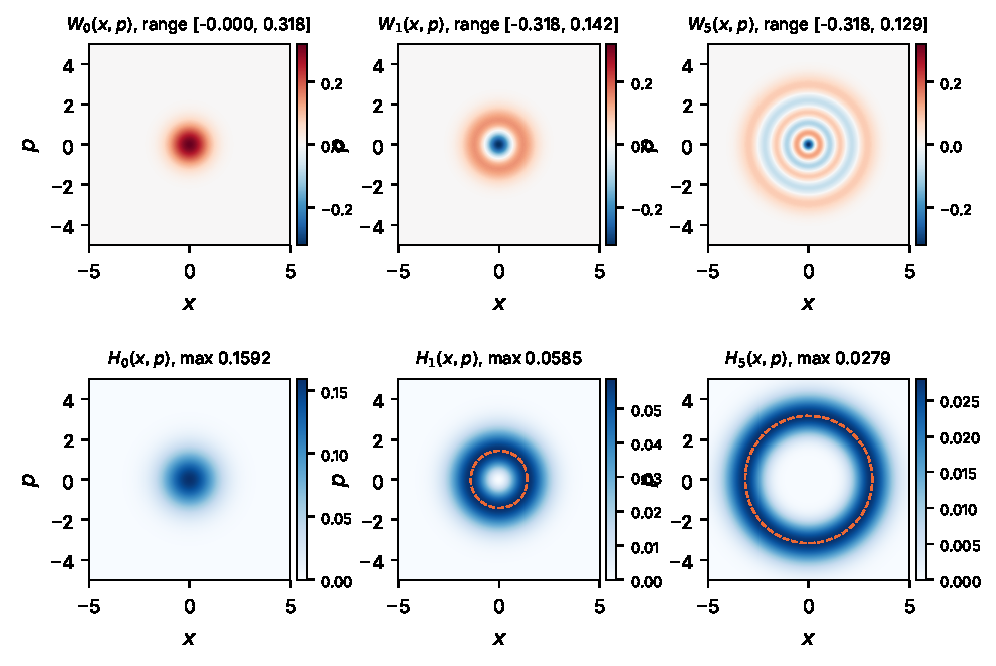
\includegraphics[width=\textwidth]{figA_wigner_husimi.pdf}
\caption{Corrected Fig.~3.2. Top: Wigner functions $W_n(x,p)$ for $n=0,1,5$ (colour range
$\pm1/\pi$). Bottom: Husimi functions $H_n(x,p)$; the dashed circle is $r=\sqrt{2n}$.
Anharmonic oscillator, $g=\lambda/4$, $\lambda=10^{-4}$.}
\label{fig:WH}
\end{figure}

\subsection{Marginals (Fig.~3.4)}
The Wigner marginal is exactly the probability density, $\rho^W_x=|\psi_n(x)|^2$. It is
symmetric about $x=0$ (for every $n$ and $\lambda$, because $|\psi_n|^2$ is even), has $n$ zeros,
and integrates to 1. The Husimi marginal is a Gaussian smoothing of it:
\begin{equation}
\rho^H_x(x)=\frac{1}{\sqrt\pi}\int e^{-(x-x')^2}|\psi_n(x')|^2\,\dd x'.
\label{eq:Hmarg}
\end{equation}
Figure~\ref{fig:marg} shows both. The thesis's Fig.~3.4 has three problems: the $n=5$
values $\sim10^{10}$ (a normalisation error), the asymmetric $n=1$ curve (a sign or parity
error in the $n=1$ state used for plotting), and the wrong number of zeros.

\begin{figure}[h]
\centering
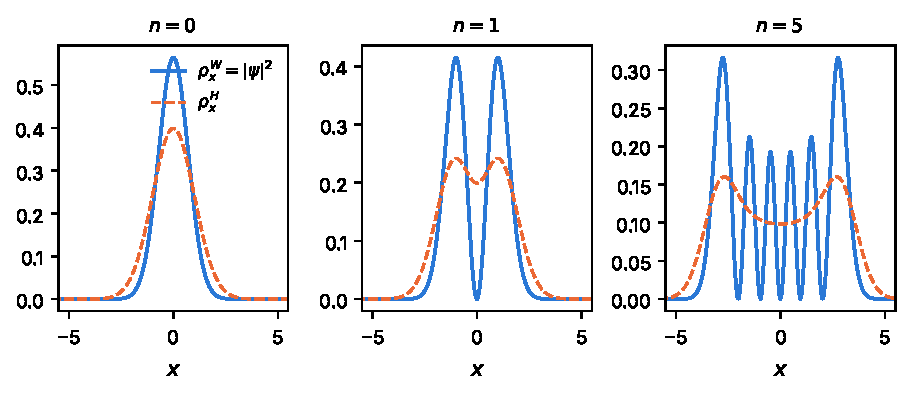
\includegraphics[width=\textwidth]{figB_marginals.pdf}
\caption{Corrected Fig.~3.4: Wigner marginal $\rho^W_x=|\psi_n|^2$ (solid) and Husimi
marginal $\rho^H_x$ (dashed) for $n=0,1,5$ ($\lambda=10^{-4}$). Both are even in $x$ and
normalised; $\rho^W_x$ has $n$ zeros.}
\label{fig:marg}
\end{figure}

\subsection{The Husimi kernel: \Eq{1.8} versus \Eq{1.9}}
\label{sec:husimi}
\Eq{1.8} smooths $W$ with $\exp[-(x-x')^2/2s^2-2s^2(p-p')^2]/\pi$. This coincides with the
coherent-state Husimi function of \Eq{1.9}, $H=|\langle\alpha|\psi\rangle|^2/2\pi$, only for
$s=1/\sqrt2$. In that case the kernel is $e^{-(x-x')^2-(p-p')^2}/\pi$, which is $x\leftrightarrow p$
symmetric with variance $1/2$ in each variable. With $s=1$ the kernel describes a squeezed
state, and the Husimi function of the HO ground state is no longer symmetric under $x\leftrightarrow p$.
This is the case in the thesis's numbers: at $\lambda=0$ the $s=1$ kernel gives
$S^H_x=1.6216$, $S^H_p=1.2751$, $S_H=2.8968$, and $S_{KL}=0.2158$ for $n=0$, whereas the
coherent-state values are $S^H_x=S^H_p=1.4189$, $S_H=1+\ln2\pi=2.8379$, and
$S_{KL}=\tfrac12(\ln2-\tfrac12)=0.0966$. \textbf{Fix:} set $s=1/\sqrt2$ in \Eq{1.8} (and state it).
Also rename this width parameter, because \S1.1.2 uses the same letter $s$ for the
Cahill--Glauber ordering parameter ($s=1,0,-1$ for $P,W,Q$), which is a different quantity.

%======================================================================
\section{Chapter 3 information measures, recomputed}
\label{sec:ch3}
%======================================================================

All quantities were recomputed from the corrected states \Eq{\ref{eq:gen}} with $g=\lambda/4$.
Exact closed forms provide checks:
\begin{itemize}
\item \textbf{Wigner Rényi-2:} $R_2^W=-\ln\!\int\!\!\int W^2=\ln2\pi=1.83788$ \emph{exactly}, for
  every pure state, every $n$ and every $\lambda$ (\Eq{\ref{eq:Wbound}}). The trends described
  in \S3.4 (``increases with $\lambda$ for $n=0$, decreases for $n=1$'') are numerical noise
  and must be removed. Our values are constant to 6 digits.
\item \textbf{Wigner Rényi-4} is \emph{not} independent of $n$: at $\lambda=0$,
  $R_4^W=\tfrac13\ln(4\pi^3)=1.607$ for $n=0$, and $1.838$ and $2.168$ for $n=1$ and $n=5$. The
  statement that $R_\alpha$ is $n$-independent for $\alpha=2$ \emph{and} $4$ is therefore
  correct only for $\alpha=2$, and only for the Wigner function. For the Husimi function,
  $R_2^H=\ln2\pi+(2n+1)\ln2-\ln\binom{2n}{n}$ depends on $n$.
\item \textbf{Wehrl entropy} at $\lambda=0$:
  $S_H=\ln2\pi+n+1+\ln n!-n\,\psi(n+1)=2.8379,\ 3.4151,\ 4.0948$ for $n=0,1,5$
  ($\psi$ is the digamma function).
\item \textbf{Wigner marginal entropies} \emph{equal} $S_x$ and $S_p$ of the wave function,
  since the marginals are identical. The phrase ``closely agree'' (Fig.~3.6) should become
  ``are identical''.
\item \textbf{Wigner Shannon entropy versus Wehrl entropy for $n=0$:}
  $-\int W_0\ln W_0=1+\ln\pi=2.1447$, while $S_H=1+\ln2\pi=2.8379$. They do \emph{not}
  coincide, contrary to \S3.4. Also, for $\lambda>0$ the ground state is not Gaussian, so by
  Hudson's theorem (quoted in \S1.1.2) its Wigner function is not strictly non-negative. The
  negativity is tiny ($|W_{\min}|<10^{-4}$) but nonzero.
\item \textbf{``Imaginary part of the WD'' (Fig.~3.13).} $W$ is real for every state, because
  $\rho$ is Hermitian. What was plotted is the imaginary part of $-\int W\ln W$ with
  $\ln W=\ln|W|+i\pi$ on $W<0$. That imaginary part equals $\pi\,\delta$, where
  $\delta=\int_{W<0}|W|$ is the Wigner negative volume (Kenfack--Życzkowski). Report
  $\delta$ directly as a non-classicality measure, and drop the language of an ``imaginary
  Wigner function''.
\item \textbf{Correlations at $\lambda=0$.} The ground state factorises, so all its
  correlation measures vanish at $\lambda=0$. For $n\ge1$ they do not vanish:
  $H_n\propto(x^2+p^2)^ne^{-(x^2+p^2)/2}$ is not a product $f(x)g(p)$. The Husimi mutual
  information is $I_H=0.0535$ ($n=1$) and $0.2702$ ($n=5$) at $\lambda=0$. The statement in
  \S3.6 must be restricted to $n=0$.
\item \textbf{Fisher information:} $F_x=4\langle p^2\rangle$ and $F_p=4\langle x^2\rangle$, equal
  to $2(2n+1)$ at $\lambda=0$.
\end{itemize}

\begin{table}[h]
\centering\small
\setlength{\tabcolsep}{4.2pt}
\begin{tabular}{@{}cc ccccccc@{}}
\toprule
$n$ & $\lambda$ & $S_x$ & $S_p$ & $S^H_x$ & $S^H_p$ & $S_H$ & $F_x$ & $F_p$\\
\midrule
0 & 0    & 1.0724 & 1.0724 & 1.4189 & 1.4189 & 2.8379 & 2.0000 & 2.0000\\
0 & 0.04 & 1.0575 & 1.0873 & 1.4116 & 1.4265 & 2.8380 & 2.0606 & 1.9415\\
0 & 0.10 & 1.0358 & 1.1092 & 1.4011 & 1.4378 & 2.8388 & 2.1536 & 1.8595\\
1 & 0    & 1.3427 & 1.3427 & 1.7343 & 1.7343 & 3.4151 & 6.0000 & 6.0000\\
1 & 0.04 & 1.3128 & 1.3615 & 1.7174 & 1.7495 & 3.4153 & 6.3042 & 5.7123\\
1 & 0.10 & 1.2693 & 1.3851 & 1.6937 & 1.7709 & 3.4168 & 6.7734 & 5.3291\\
5 & $10^{-4}$ & 1.7678 & 1.7681 & 2.1824 & 2.1826 & 4.0948 & 22.009 & 21.991\\
\midrule
$n$ & $\lambda$ & $R^W_2$ & $R^W_4$ & $R^H_2$ & $R^H_4$ & $S_{KL}(\rho_x\|\rho^H_x)$ & $D_{CS}(W,H)$ & $I_H$\\
\midrule
0 & 0    & 1.8379 & 1.6068 & 2.5310 & 2.3000 & 0.0966 & 0.0589 & 0.0000\\
0 & 0.04 & 1.8379 & 1.6068 & 2.5312 & 2.3001 & 0.1006 & 0.0589 & 0.0000\\
0 & 0.10 & 1.8379 & 1.6069 & 2.5318 & 2.3008 & 0.1067 & 0.0592 & 0.0001\\
1 & 0    & 1.8379 & 1.8379 & 3.2242 & 3.0890 & 0.2042 & 0.3001 & 0.0535\\
1 & 0.04 & 1.8379 & 1.8379 & 3.2242 & 3.0888 & 0.2145 & 0.3003 & 0.0515\\
1 & 0.10 & 1.8379 & 1.8379 & 3.2247 & 3.0876 & 0.2304 & 0.3013 & 0.0479\\
5 & $10^{-4}$ & 1.8379 & 2.1675 & 3.9331 & 3.8134 & 0.2849 & 0.6938 & 0.2702\\
\bottomrule
\end{tabular}
\caption{Corrected Chapter~3 measures (coherent-state Husimi function, $g=\lambda/4$).
$I_H=S^H_x+S^H_p-S_H$. $D_{CS}=-\ln[\int WH/(\int W^2\int H^2)^{1/2}]$.
Every $\lambda=0$ entry agrees with its closed form.}
\label{tab:ch3}
\end{table}

\begin{figure}[h]
\centering
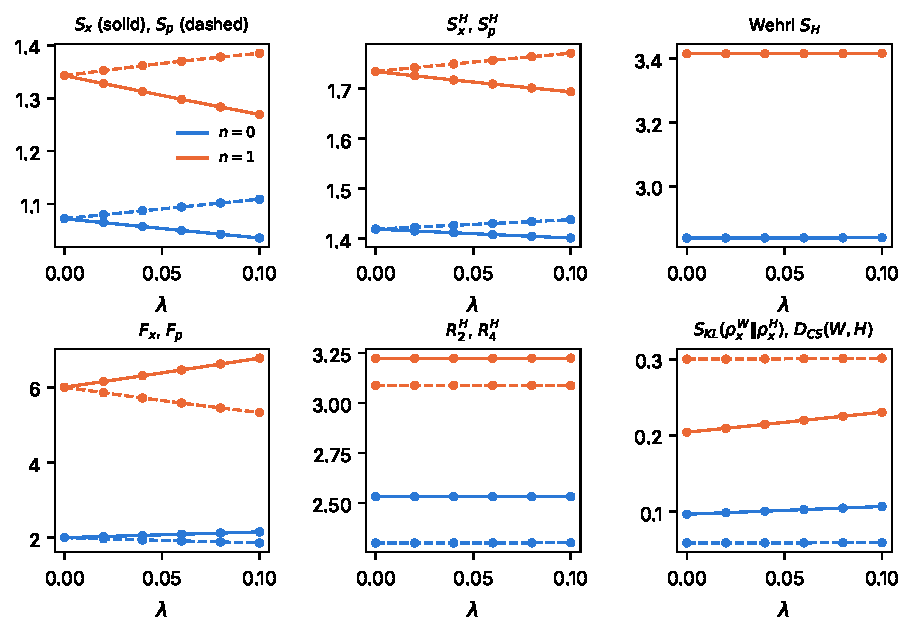
\includegraphics[width=\textwidth]{figC_ch3_measures.pdf}
\caption{Corrected Chapter~3 measures versus $\lambda$ for $n=0$ and $n=1$ (replaces the
curves in Figs.~3.6--3.10, 3.12). Note that $R^W_2=\ln2\pi$ is constant.}
\label{fig:ch3}
\end{figure}

\paragraph{Trends that change.} (i) $D_{CS}$ \emph{increases} slightly with $\lambda$ for
both states; the thesis says it decreases. (ii) $I_H$ for $n=1$ \emph{decreases} with
$\lambda$. (iii) $S_{KL}$ increases with both $\lambda$ and $n$, as the thesis states.
The survival functions, cumulative residual entropies, Jeffreys divergence, Rényi
divergences, and CCRE (Figs.~3.3, 3.5, 3.10, 3.11, 3.13) use the same distributions and
must be regenerated from them. Their definitions need no change.

%======================================================================
\section{Chapter 4, quartic potential: corrected Tables 4.1 and 4.3}
\label{sec:q}
%======================================================================

Because first order fails at $b\ge1$ (Table~\ref{tab:fid}), Tables~4.1 and 4.3 were
recomputed by exact diagonalisation. We used a sinc discrete-variable representation (DVR)
on $[-7,7]$ with 401 points, which converges energies to $10^{-10}$. $F_x$ was computed as
$8(E-\langle V\rangle)$ and $F_k$ as $4\langle x^2\rangle$. Small-$b$ first-order values are
included for comparison.

\begin{table}[h]
\centering\small
\begin{tabular}{@{}cc ccc ccc@{}}
\toprule
& & \multicolumn{3}{c}{thesis Table 4.1} & \multicolumn{3}{c}{exact}\\
\cmidrule(lr){3-5}\cmidrule(l){6-8}
$n$ & $b$ & $S_x$ & $S_k$ & $S_x+S_k$ & $S_x$ & $S_k$ & $S_x+S_k$\\
\midrule
0 & 1   & \Th{1.6454} & \Th{1.3977} & \Th{3.0431} & 0.7383 & 1.4108 & 2.1491\\
  & 1.3 & \Th{1.6417} & \Th{1.4193} & \Th{3.0610} & 0.7028 & 1.4467 & 2.1495\\
  & 1.5 & \Th{1.6382} & \Th{1.4279} & \Th{3.0662} & 0.6829 & 1.4667 & 2.1497\\
1 & 1   & \Th{1.3151} & \Th{1.2521} & \Th{2.5672} & 0.8985 & 1.7306 & 2.6290\\
  & 1.3 & \Th{1.4247} & \Th{1.2262} & \Th{2.6509} & 0.8595 & 1.7682 & 2.6277\\
  & 1.5 & \Th{1.4840} & \Th{1.2333} & \Th{2.7172} & 0.8379 & 1.7891 & 2.6271\\
2 & 1   & \Th{1.3317} & \Th{1.6758} & \Th{3.0075} & 1.0002 & 1.8911 & 2.8912\\
  & 1.3 & \Th{1.3638} & \Th{1.9453} & \Th{3.3091} & 0.9604 & 1.9284 & 2.8888\\
  & 1.5 & \Th{1.1718} & \Th{1.9459} & \Th{3.1177} & 0.9383 & 1.9492 & 2.8875\\
3 & 1   & \Th{1.3459} & \Th{1.5482} & \Th{2.8941} & 1.0730 & 2.0057 & 3.0787\\
  & 1.3 & \Th{1.3879} & \Th{1.7297} & \Th{3.1175} & 1.0325 & 2.0432 & 3.0757\\
  & 1.5 & \Th{1.2038} & \Th{1.6589} & \Th{2.8625} & 1.0103 & 2.0641 & 3.0744\\
\midrule
\multicolumn{8}{l}{small $b$: exact (first order) \quad [$S_x+S_k\ge1+\ln\pi=2.1447$ in all cases]}\\
0 & 0.01 & \multicolumn{3}{c}{} & 1.0583 (1.0575) & 1.0864 (1.0873) & 2.1448 (2.1448)\\
0 & 0.10 & \multicolumn{3}{c}{} & 0.9758 (0.9443) & 1.1698 (1.2101) & 2.1456 (2.1544)\\
1 & 0.01 & \multicolumn{3}{c}{} & 1.3159 (1.3128) & 1.3613 (1.3616) & 2.6772 (2.6744)\\
3 & 0.01 & \multicolumn{3}{c}{} & 1.5633 (1.5498) & 1.6310 (1.6250) & 3.1943 (3.1748)\\
\bottomrule
\end{tabular}
\caption{Corrected Table~4.1 (quartic, Shannon entropies). Thesis values in red.}
\label{tab:q41}
\end{table}

\begin{table}[h]
\centering\small
\setlength{\tabcolsep}{4.5pt}
\begin{tabular}{@{}cc ccc ccccc@{}}
\toprule
& & \multicolumn{3}{c}{thesis Table 4.3} & \multicolumn{5}{c}{exact}\\
\cmidrule(lr){3-5}\cmidrule(l){6-10}
$n$ & $b$ & $F_x$ & $F_k$ & $F_xF_k$ & $F_x$ & $F_k$ & $\sigma_x^2$ & $\sigma_k^2$ & $F_xF_k$\\
\midrule
0 & 1   & \Th{8.256} & \Th{13.07} & \Th{107.9} & 3.9439 & 1.0286 & 0.2571 & 0.9860 & 4.057\\
  & 1.3 & \Th{8.100} & \Th{13.65} & \Th{110.6} & 4.2380 & 0.9583 & 0.2396 & 1.0595 & 4.061\\
  & 1.5 & \Th{8.018} & \Th{13.90} & \Th{111.4} & 4.4119 & 0.9211 & 0.2303 & 1.1030 & 4.064\\
1 & 1   & \Th{12.38} & \Th{6.000} & \Th{74.31} & 13.718 & 2.6517 & 0.6629 & 3.4295 & 36.38\\
  & 1.3 & \Th{13.11} & \Th{7.434} & \Th{97.46} & 14.806 & 2.4584 & 0.6146 & 3.7014 & 36.40\\
  & 1.5 & \Th{13.37} & \Th{8.359} & \Th{111.8} & 15.446 & 2.3572 & 0.5893 & 3.8615 & 36.41\\
2 & 1   & \Th{12.82} & \Th{9.567} & \Th{122.6} & 26.366 & 3.7699 & 0.9425 & 6.5916 & 99.40\\
  & 1.3 & \Th{21.66} & \Th{16.17} & \Th{350.2} & 28.546 & 3.4803 & 0.8701 & 7.1364 & 99.35\\
  & 1.5 & \Th{28.84} & \Th{21.52} & \Th{405.5} & 29.825 & 3.3301 & 0.8325 & 7.4563 & 99.32\\
3 & 1   & \Th{6.039} & \Th{3.235} & \Th{19.53} & 40.772 & 4.7623 & 1.1906 & 10.193 & 194.2\\
  & 1.3 & \Th{10.21} & \Th{5.466} & \Th{55.79} & 44.210 & 4.3899 & 1.0975 & 11.053 & 194.1\\
  & 1.5 & \Th{13.59} & \Th{7.278} & \Th{98.88} & 46.226 & 4.1975 & 1.0494 & 11.556 & 194.0\\
\bottomrule
\end{tabular}
\caption{Corrected Table~4.3 (quartic, Fisher information). Thesis values in red. Within
the thesis's table, $n=2$, $b=1.5$ violates its own relation $F_x=4\sigma_k^2$
($28.84\ne4\times4.7095$).}
\label{tab:q43}
\end{table}

\paragraph{What changes in the discussion of \S4.4.}
\begin{itemize}
\item $S_x$ decreases and $S_k$ increases with $b$ for \emph{every} $n$. The thesis text says
  this, but its own Table~4.1 shows $S_x$ \emph{increasing} for $n=1$.
\item $S_x+S_k$ is \emph{not} independent of $b$. For $n=0$ it rises from $1+\ln\pi=2.1447$
  at $b=0$ to $2.1497$ at $b=1.5$. For $n=1$, 2 and 3 it falls from the HO values $2.6854$,
  $2.9972$ and $3.2194$ at $b=0$ to $2.627$, $2.888$ and $3.074$ at $b=1.5$. \Eq{4.20} is false.
\item The Fisher informations are \emph{not} ``nearly constant'' (\S4.4.2): $F_x$ more than
  doubles for every $n$ between $b=0$ and $b=1.5$ (e.g.\ $2\to4.41$ for $n=0$), while $F_k$
  falls by a factor of $2$--$3.5$. $F_xF_k\approx4(2n+1)^2$ remains close to its HO value.
\item Figures 4.7 and 4.9 must be replaced by the top half of Fig.~\ref{fig:ch4}.
\end{itemize}

\begin{figure}[p]
\centering
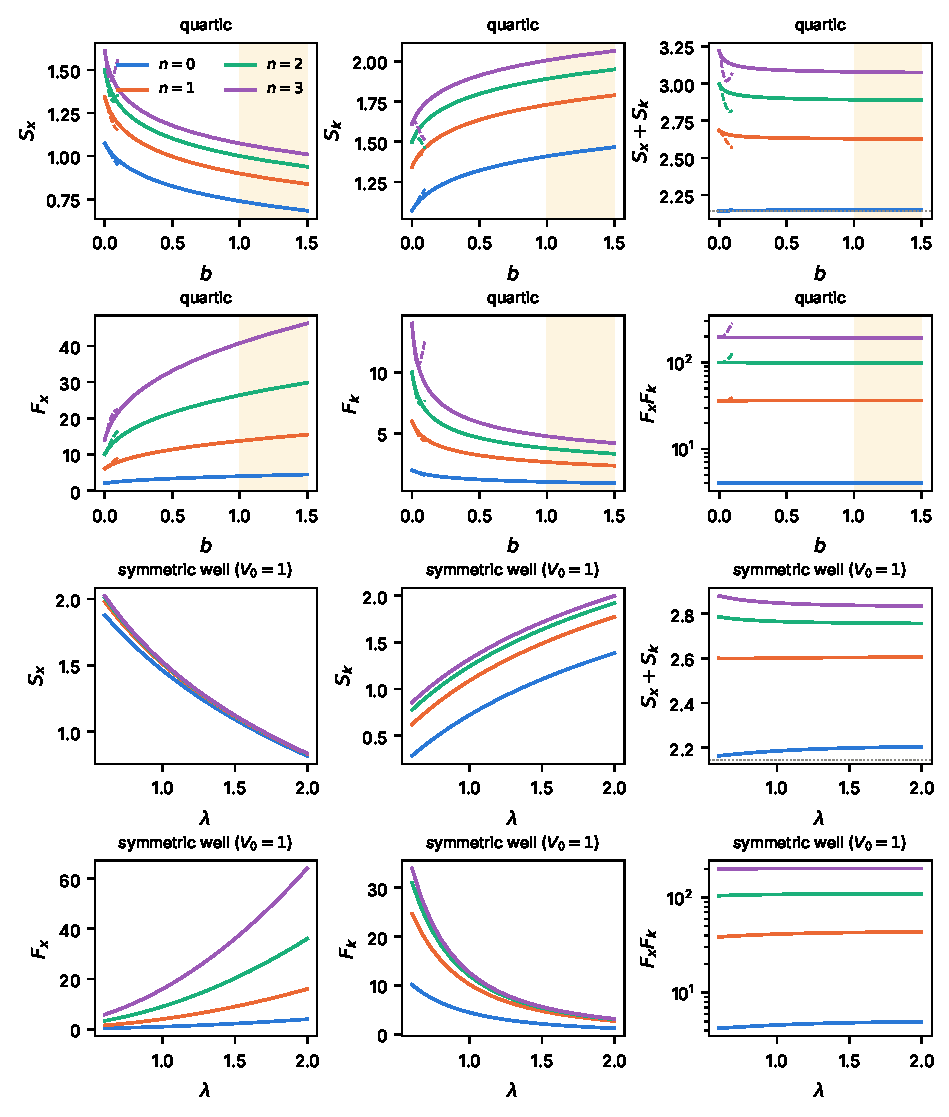
\includegraphics[width=0.97\textwidth]{figE_ch4_exact.pdf}
\caption{Corrected Figs.~4.7--4.10 (exact diagonalisation, $n=0$ blue, 1 orange, 2 green, 3
purple). Rows 1--2: quartic potential versus $b$. Dashed lines are first order, shown for
$b\le0.1$; the shaded band is the range of the thesis's tables. Rows 3--4: symmetric well
($V_0=1$) versus $\lambda$. Neither $S_x+S_k$ nor $F_xF_k$ is constant.}
\label{fig:ch4}
\end{figure}

%======================================================================
\section{Chapter 4, symmetric well: the scaling error and corrected Tables 4.2 and 4.4}
\label{sec:well}
%======================================================================

\subsection{The potential and its exact ground state}
$V(x)=V_0\,\dfrac{1-\lambda x\cot\lambda x}{(\lambda x)^2}$ is a \emph{single} well with
infinite walls at $|x|=\pi/\lambda$ (where $\cot\lambda x\to\mp\infty$). Near the origin,
$V=V_0[\tfrac13+\tfrac{(\lambda x)^2}{45}+\tfrac{2(\lambda x)^4}{945}+\tfrac{(\lambda x)^6}{4725}+\dots]$,
and this series converges only for $|\lambda x|<\pi$. Direct differentiation shows that for
$V_0=\lambda^2$ the ground state is known in closed form:
\begin{equation}
\psi_0(x)=\frac{\sin\lambda x}{x\sqrt{2\lambda\,\Si(2\pi)}},\qquad E_0=\frac{\lambda^2}{2},\qquad |x|<\pi/\lambda,
\label{eq:sinc}
\end{equation}
since $-\tfrac12\psi_0''/\psi_0=\tfrac{\lambda^2}{2}-\tfrac{1-\lambda x\cot\lambda x}{x^2}$.
For $V_0=1$ (the thesis's choice) this is exact at $\lambda=1$, which gives an exact
benchmark: $F_k=4\langle x^2\rangle=2\pi/\Si(2\pi)=4.43055$, $F_x=1.03406$, and $S_x=1.46124$.
Our DVR reproduces these to $10^{-5}$ ($E_0=0.4999998$, overlap $1-5\times10^{-13}$).

\subsection{The error in Appendix A3}
Put $\chi=\lambda x$ in $-\tfrac12\psi''+V_0g(\lambda x)\psi=E\psi$:
\begin{equation}
-\tfrac12\,\frac{\dd^2\phi}{\dd\chi^2}+\frac{V_0}{\lambda^2}\,g(\chi)\,\phi=\frac{E}{\lambda^2}\,\phi .
\label{eq:chi}
\end{equation}
\Eq{A3.4} sets $V_0=1$ but omits the factor $1/\lambda^2$ in front of the potential. That is
the same as taking $V_0=\lambda^2$. The $\chi$-equation then contains no $\lambda$, every
state has the form $\psi(x)=\sqrt\lambda\,f(\lambda x)$, and it follows identically that
\begin{equation}
S_x(\lambda)=S_x(1)-\ln\lambda,\quad S_k(\lambda)=S_k(1)+\ln\lambda,\quad F_x\propto\lambda^2,\quad F_k\propto\lambda^{-2}.
\label{eq:scaling}
\end{equation}
Tables~4.2 and 4.4 show exactly this pattern. For $n=2$, $S_x(1)-S_x(1.3)=0.26236=\ln1.3$
and $S_x(1)-S_x(1.5)=0.40546=\ln1.5$; $S_x+S_k=2.77544$ at all three $\lambda$; and
$F_xF_k=211.9158$ at all three. So the ``$\lambda$-independence'' of \Eq{4.20} reflects this
error: in the thesis's own model $\lambda$ is only a length unit. Further consequences:
\begin{itemize}
\item The Gaussian in \Eq{4.16} and (A3.15) is $e^{-\lambda^2x^2/3\sqrt{10}}$. For $V_0=1$ the
  oscillator frequency is $\omega=\lambda\sqrt{2/45}$, so the Gaussian must be
  $e^{-\omega x^2/2}=e^{-\lambda x^2/3\sqrt{10}}$, and the Hermite argument must be
  $y=\sqrt\omega\,x=(2/45)^{1/4}\sqrt\lambda\,x$ rather than one $\propto\lambda x$.
\item \Eq{A3.14} keeps only the $x^4$ part of the perturbation. Its coefficients
  $-0.0847\sqrt8=-3\sqrt5/28$ and $-0.0035\sqrt{384}\approx-\sqrt{15}/56$ are exactly the
  $\beta_4$ terms below. The $x^6$ term $\beta_6$, of the same order, is dropped there but
  kept in (A3.17) for $n=2$, so the truncation is inconsistent.
\item \Eq{4.18} for $n=1$ contains the constant $0.508967$ alongside odd terms, so it has
  mixed parity. Its Fourier transform \Eq{4.19} accordingly has the real constant $1.1084$
  next to imaginary odd terms. This is the same defect as in Eqs.~(4.12)--(4.13), and the
  same cure applies (\S\ref{sec:parity}). The normalisations $C_1$ (with $10^{-12}$ terms)
  and $D_1$ (a polynomial in $\lambda$ up to $\lambda^{11}$) are artefacts of it.
\item Table~4.4 gives $\sigma_x^2=22.3$, $14.0$, $10.3$ at $\lambda=1$ for $n=1,2,3$. The particle
  is confined to $|x|<\pi$, so $\sigma_x^2<\pi^2=9.87$. These values are impossible. They
  arise because the truncated $x^6$ polynomial has no walls.
\end{itemize}

\subsection{Correct first-order states (for completeness)}
Write $\mu=\lambda/\sqrt{V_0}$. The $x^6$-truncated Hamiltonian is
\begin{equation}
H=\tfrac{V_0}{3}+\omega\left(a^\dagger a+\tfrac12\right)+\omega\left(\beta_4y^4+\beta_6y^6\right),\qquad
\omega=\lambda\sqrt{\tfrac{2V_0}{45}},\quad \beta_4=\tfrac{\sqrt{10}}{14}\mu,\quad \beta_6=\tfrac{3}{28}\mu^2,
\label{eq:Hwell}
\end{equation}
with $y=\sqrt\omega\,x=(a+a^\dagger)/\sqrt2$. The relative strength of the perturbation depends
only on $\mu$: for $V_0=1$, $\mu=\lambda$; for the thesis's effective $V_0=\lambda^2$, $\mu=1$
for every $\lambda$. The first-order states and energies are
\begin{align*}
\ket{\psi_0}&\propto\ket0-\frac{3\mu(45\sqrt2\mu+16\sqrt5)}{448}\ket2-\frac{\mu(45\sqrt6\mu+8\sqrt{15})}{448}\ket4-\frac{3\sqrt5\mu^2}{112}\ket6,\\
\ket{\psi_1}&\propto\ket1-\frac{5\mu(63\sqrt6\mu+16\sqrt{15})}{448}\ket3-\frac{\mu(63\sqrt{30}\mu+40\sqrt3)}{448}\ket5-\frac{3\sqrt{35}\mu^2}{112}\ket7,\\
\ket{\psi_2}&\propto\ket2+\frac{3\mu(45\sqrt2\mu+16\sqrt5)}{448}\ket0-\frac{\mu(585\sqrt3\mu+56\sqrt{30})}{224}\ket4\\
&\qquad-\frac{3\mu(81\sqrt{10}\mu+40)}{448}\ket6-\frac{3\sqrt{35}\mu^2}{56}\ket8,\\
\ket{\psi_3}&\propto\ket3+\frac{5\mu(63\sqrt6\mu+16\sqrt{15})}{448}\ket1-\frac{45\mu(21\sqrt5\mu+8\sqrt2)}{224}\ket5\\
&\qquad-\frac{\mu(99\sqrt{210}\mu+40\sqrt{21})}{448}\ket7-\frac{3\sqrt{105}\mu^2}{56}\ket9,
\end{align*}
\begin{gather*}
\frac{E_0-V_0/3}{\omega}=\frac12+\frac{3\sqrt{10}}{56}\mu+\frac{45}{224}\mu^2,\qquad
\frac{E_1-V_0/3}{\omega}=\frac32+\frac{15\sqrt{10}}{56}\mu+\frac{45}{32}\mu^2,\\
\frac{E_2-V_0/3}{\omega}=\frac52+\frac{39\sqrt{10}}{56}\mu+\frac{1125}{224}\mu^2,\qquad
\frac{E_3-V_0/3}{\omega}=\frac72+\frac{75\sqrt{10}}{56}\mu+\frac{405}{32}\mu^2.
\end{gather*}
Each state contains only $\ket m$ with $m\equiv n\pmod2$, so $\psi_n$ has parity $(-1)^n$. In
coordinates, $\langle x|m\rangle=(\omega/\pi)^{1/4}(2^mm!)^{-1/2}H_m(y)e^{-y^2/2}$ and
$\langle k|m\rangle=(-i)^m(\pi\omega)^{-1/4}(2^mm!)^{-1/2}H_m(q)e^{-q^2/2}$ with $q=k/\sqrt\omega$. For
example, the corrected $n=1$ state replacing Eqs.~(4.18)--(4.19) is
\begin{align}
\psi_1(x)&=N_1\Big(\frac\omega\pi\Big)^{1/4}e^{-y^2/2}\,y\Big[\sqrt2+\frac{45\sqrt5}{112}\mu+\frac{165\sqrt2}{128}\mu^2
-\Big(\frac{5\sqrt5}{28}\mu+\frac{15\sqrt2}{32}\mu^2\Big)y^2\nonumber\\
&\hspace{6cm}-\Big(\frac{\sqrt5}{28}\mu+\frac{3\sqrt2}{32}\mu^2\Big)y^4-\frac{\sqrt2}{56}\mu^2y^6\Big],\nonumber\\
\varphi_1(k)&=-i\,N_1(\pi\omega)^{-1/4}e^{-q^2/2}\,q\Big[\sqrt2-\frac{75\sqrt5}{112}\mu-\frac{435\sqrt2}{128}\mu^2
+\Big(\frac{15\sqrt5}{28}\mu+\frac{105\sqrt2}{32}\mu^2\Big)q^2\nonumber\\
&\hspace{6cm}-\Big(\frac{\sqrt5}{28}\mu+\frac{15\sqrt2}{32}\mu^2\Big)q^4+\frac{\sqrt2}{56}\mu^2q^6\Big],\nonumber\\
N_1^{-2}&=1+\frac{225}{448}\mu^2+\frac{1485\sqrt{10}}{1792}\mu^3+\frac{25695}{7168}\mu^4 .
\label{eq:well1}
\end{align}
$\psi_1$ is odd and $\varphi_1$ is $-i$ times an odd real function. The other normalisations are
\begin{gather*}
N_0^{-2}=1+\frac{195}{3136}\mu^2+\frac{135\sqrt{10}}{1792}\mu^3+\frac{6165}{25088}\mu^4,\qquad
N_2^{-2}=1+\frac{6285}{3136}\mu^2+\frac{53595\sqrt{10}}{12544}\mu^3+\frac{594225}{25088}\mu^4,\\
N_3^{-2}=1+\frac{18225}{3136}\mu^2+\frac{27135\sqrt{10}}{1792}\mu^3+\frac{734805}{7168}\mu^4.
\end{gather*}

\paragraph{But first order is not adequate here.} At $\mu=1$ the mixing coefficients are of
order one ($c_2\approx-0.67$ for $n=0$). Table~\ref{tab:wfid} compares the first-order
states with the exact eigenstates of the truncated $x^6$ model and of the full potential.
The $x^6$ truncation also changes the physics, because the walls at $\pi/\lambda$ are lost.
\textbf{Recommendation:} drop the perturbative treatment of this potential and diagonalise
the full potential on $(-\pi/\lambda,\pi/\lambda)$ with Dirichlet walls.

\begin{table}[h]
\centering\small
\begin{tabular}{@{}c cccc cccc@{}}
\toprule
& \multicolumn{4}{c}{overlap with exact state of $x^6$ model} & \multicolumn{4}{c}{overlap with exact state of full $V$}\\
\cmidrule(lr){2-5}\cmidrule(l){6-9}
$\lambda$ ($V_0=1$) & $n=0$ & 1 & 2 & 3 & $n=0$ & 1 & 2 & 3\\
\midrule
0.5 & 0.978 & 0.796 & 0.557 & 0.471 & 0.998 & 0.992 & 0.982 & 0.820\\
1.0 & 0.774 & 0.384 & 0.319 & 0.319 & 1.000 & 0.975 & 0.781 & 0.488\\
1.5 & 0.478 & 0.250 & 0.260 & 0.246 & 0.999 & 0.902 & 0.648 & 0.194\\
2.0 & 0.294 & 0.203 & 0.230 & 0.195 & 0.995 & 0.841 & 0.545 & 0.027\\
\bottomrule
\end{tabular}
\caption{Symmetric well: overlap $|\langle\psi^{\rm exact}|\psi^{(1)}\rangle|^2$ of the first-order
states \Eq{\ref{eq:Hwell}}. The good $n=0$ overlap with the full potential is fortuitous: the
same state is a poor approximation to the model it was derived from.}
\label{tab:wfid}
\end{table}

\subsection{Corrected Tables 4.2 and 4.4 (exact, $V_0=1$)}
We computed exact eigenstates with a box DVR on $(-\pi/\lambda,\pi/\lambda)$ (600 points),
evaluating $F_x$ as $8(E-\langle V\rangle)$. At $\lambda=1$ both readings of the model ($V_0=1$
and $V_0=\lambda^2$) coincide, so the thesis's $\lambda=1$ rows can be compared directly. For
$V_0=\lambda^2$, all other $\lambda$ follow from the $\lambda=1$ row by \Eq{\ref{eq:scaling}}.

\begin{table}[h]
\centering\small
\begin{tabular}{@{}cc c ccc ccc@{}}
\toprule
& & & \multicolumn{3}{c}{thesis Table 4.2} & \multicolumn{3}{c}{exact ($V_0=1$)}\\
\cmidrule(lr){4-6}\cmidrule(l){7-9}
$n$ & $\lambda$ & $E_n$ & $S_x$ & $S_k$ & $S_x+S_k$ & $S_x$ & $S_k$ & $S_x+S_k$\\
\midrule
0 & 1   & 0.5000 & \Th{1.6545} & \Th{0.5575} & \Th{2.2120} & 1.4612 & 0.7233 & 2.1846\\
  & 1.3 & 0.5881 & \Th{1.3922} & \Th{0.8197} & \Th{2.2118} & 1.2256 & 0.9681 & 2.1937\\
  & 1.5 & 0.6588 & \Th{1.2491} & \Th{0.9627} & \Th{2.2117} & 1.0928 & 1.1049 & 2.1976\\
  & 2   & 0.8786 & -- & -- & -- & 0.8191 & 1.3844 & 2.2034\\
1 & 1   & 0.9421 & \Th{2.3534} & \Th{0.2965} & \Th{2.6499} & 1.5095 & 1.0910 & 2.6005\\
  & 1.3 & 1.2907 & \Th{1.8103} & \Th{0.5589} & \Th{2.3691} & 1.2564 & 1.3460 & 2.6024\\
  & 1.5 & 1.5720 & \Th{1.5690} & \Th{0.7019} & \Th{2.2708} & 1.1165 & 1.4869 & 2.6033\\
  & 2   & 2.4489 & -- & -- & -- & 0.8329 & 1.7719 & 2.6048\\
2 & 1   & 1.6102 & \Th{1.9907} & \Th{0.7847} & \Th{2.7754} & 1.5209 & 1.2438 & 2.7648\\
  & 1.3 & 2.3895 & \Th{1.7284} & \Th{1.0471} & \Th{2.7754} & 1.2630 & 1.4970 & 2.7600\\
  & 1.5 & 3.0206 & \Th{1.5853} & \Th{1.1902} & \Th{2.7754} & 1.1214 & 1.6369 & 2.7583\\
  & 2   & 4.9909 & -- & -- & -- & 0.8356 & 1.9204 & 2.7560\\
3 & 1   & 2.5161 & \Th{1.7691} & \Th{0.8380} & \Th{2.6072} & 1.5253 & 1.3222 & 2.8475\\
  & 1.3 & 3.8985 & \Th{1.5068} & \Th{1.1004} & \Th{2.6072} & 1.2655 & 1.5745 & 2.8400\\
  & 1.5 & 5.0194 & \Th{1.3637} & \Th{1.2435} & \Th{2.6072} & 1.1232 & 1.7140 & 2.8373\\
  & 2   & 8.5206 & -- & -- & -- & 0.8366 & 1.9970 & 2.8336\\
\bottomrule
\end{tabular}
\caption{Corrected Table~4.2 (symmetric well, Shannon entropies). Thesis values in red.
$E_0(\lambda=1)=1/2$ exactly (\Eq{\ref{eq:sinc}}).}
\label{tab:w42}
\end{table}

\begin{table}[h]
\centering\small
\setlength{\tabcolsep}{4.5pt}
\begin{tabular}{@{}cc ccc ccccc@{}}
\toprule
& & \multicolumn{3}{c}{thesis Table 4.4} & \multicolumn{5}{c}{exact ($V_0=1$)}\\
\cmidrule(lr){3-5}\cmidrule(l){6-10}
$n$ & $\lambda$ & $F_x$ & $F_k$ & $F_xF_k$ & $F_x$ & $F_k$ & $\sigma_x^2$ & $\sigma_k^2$ & $F_xF_k$\\
\midrule
0 & 1   & \Th{0.7515} & \Th{6.833} & \Th{5.135} & 1.0341 & 4.4306 & 1.1076 & 0.2585 & 4.581\\
  & 1.3 & \Th{1.270}  & \Th{4.043} & \Th{5.135} & 1.7129 & 2.7770 & 0.6942 & 0.4282 & 4.757\\
  & 1.5 & \Th{1.691}  & \Th{3.037} & \Th{5.135} & 2.2680 & 2.1327 & 0.5332 & 0.5670 & 4.837\\
1 & 1   & \Th{0.6920} & \Th{89.12} & \Th{61.67} & 4.0665 & 10.155 & 2.5388 & 1.0166 & 41.30\\
  & 1.3 & \Th{0.8996} & \Th{52.73} & \Th{47.44} & 6.8030 & 6.2342 & 1.5586 & 1.7008 & 42.41\\
  & 1.5 & \Th{1.038}  & \Th{39.61} & \Th{41.11} & 9.0334 & 4.7479 & 1.1870 & 2.2583 & 42.89\\
2 & 1   & \Th{3.786}  & \Th{55.98} & \Th{211.9} & 9.0590 & 11.912 & 2.9779 & 2.2648 & 107.9\\
  & 1.3 & \Th{6.398}  & \Th{33.12} & \Th{211.9} & 15.246 & 7.1432 & 1.7858 & 3.8115 & 108.9\\
  & 1.5 & \Th{8.518}  & \Th{24.88} & \Th{211.9} & 20.277 & 5.3893 & 1.3473 & 5.0693 & 109.3\\
3 & 1   & \Th{2.238}  & \Th{41.13} & \Th{92.05} & 16.048 & 12.568 & 3.1420 & 4.0120 & 201.7\\
  & 1.3 & \Th{3.783}  & \Th{24.34} & \Th{92.05} & 27.068 & 7.4672 & 1.8668 & 6.7671 & 202.1\\
  & 1.5 & \Th{5.036}  & \Th{18.28} & \Th{92.05} & 36.021 & 5.6150 & 1.4037 & 9.0053 & 202.3\\
\bottomrule
\end{tabular}
\caption{Corrected Table~4.4 (symmetric well, Fisher information). Thesis values in red. The
thesis's $\sigma_x^2$ values for $n=1,2,3$ at $\lambda=1$ (22.3, 14.0, 10.3) exceed the bound $\pi^2$.}
\label{tab:w44}
\end{table}

\clearpage
\paragraph{What changes in the discussion.}
\begin{itemize}
\item \Eq{4.20} is false for the stated model. With $V_0=1$, over $\lambda\in[0.6,2]$, $S_x+S_k$
  varies by $0.040$ for $n=0$ (2.163--2.203) and $F_xF_k$ varies from $4.23$ to $4.96$
  (Fig.~\ref{fig:ch4}). With $V_0=\lambda^2$ the constancy holds, but only because $\lambda$
  is then a pure length scale, which has no physical content.
\item \S4.4.2 says that $F_x$ \emph{decreases} as localisation in position increases. Both
  the exact results and the thesis's own Table~4.4 show $F_x$ \emph{increasing} with $\lambda$
  (stronger confinement), with $F_k$ decreasing.
\item The interpretation via Boltzmann's H-theorem (\S4.4.2) has no basis. These are
  stationary states of a closed system with no dynamics and no approach to equilibrium.
  Delete it.
\end{itemize}

%======================================================================
\section{Overall approach (examiner's closing comments)}
\label{sec:overall}
%======================================================================

The examiner suggests exact numerical diagonalisation for many states. This is cheap: each
panel of Fig.~\ref{fig:many}(b) takes seconds, with 1200 grid points. The figure shows
$S_x+S_k$ for all even states up to $n=100$. For the quartic oscillator ($b=1$) the sum grows
logarithmically. The semiclassical estimate gives $S_x+S_k\simeq\ln n+{}$const for any
power-law well, and the local slope is already $0.76$ at $n=50$--$100$. For the
symmetric well it saturates at $3.060$, the value for a particle in an infinite square well
(which we checked: $3.0598$ at $n=101$). The highly excited states feel only the walls.
Such results, together with the semiclassical limit of the Husimi distribution (which
concentrates on the classical orbit $H(x,p)=E_n$), would make Chapter~4 substantially more
interesting than a few perturbative states.

\begin{figure}[h]
\centering
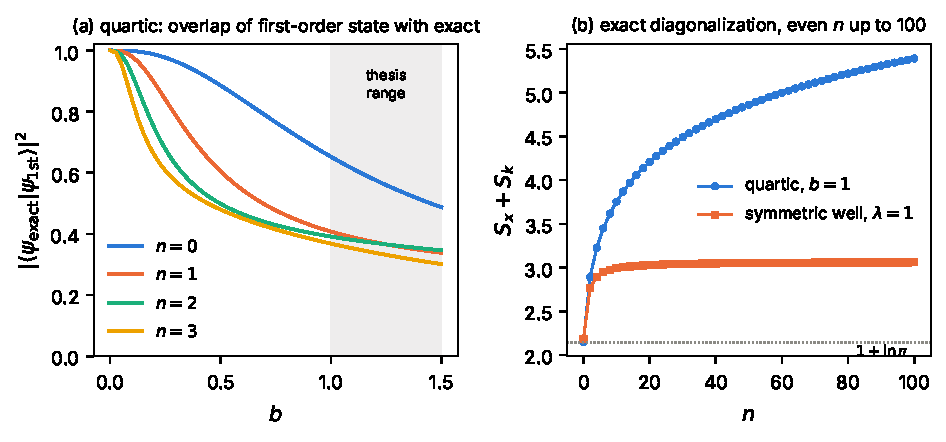
\includegraphics[width=\textwidth]{figD_validity_many.pdf}
\caption{(a) Quartic oscillator: overlap of the first-order state with the exact state.
The shaded band is the thesis's range $b=1$--$1.5$. (b) $S_x+S_k$ from exact diagonalisation
for even $n\le100$: quartic potential $b=1$ and symmetric well $\lambda=1$, $V_0=1$.}
\label{fig:many}
\end{figure}

\paragraph{Suggested restructuring.}
\begin{enumerate}
\item Merge Chapter~3 and \S4.2 into one chapter on $H=p^2/2+x^2/2+gx^4$. Give the general
  first-order state \Eq{\ref{eq:gen}} once, use it only for $g\lesssim0.05$, and use exact
  diagonalisation otherwise.
\item Treat the symmetric well with the full potential and exact diagonalisation. Use the
  exact solution \Eq{\ref{eq:sinc}} as the benchmark.
\item Report the Wigner negative volume and $R_2$-type measures, which are well defined,
  instead of complex Shannon entropies of $W$.
\item Add the many-state analysis (Fig.~\ref{fig:many}b) and its semiclassical
  interpretation. A natural extension beyond 1D, also mentioned by the examiner, is two
  coupled oscillators, for which the same phase-space measures quantify entanglement.
\end{enumerate}

%======================================================================
\section{Checklist of changes to the thesis}
\label{sec:checklist}
%======================================================================

\begin{enumerate}[label=\arabic*.,leftmargin=1.6em]
\item \textbf{\Eq{1.7}}: $\langle\hat O\rangle=\int\!\!\int O_W(x,p)W(x,p)\,\dd x\,\dd p$, without
  $2\pi$. The factor $2\pi$ belongs to $\operatorname{Tr}(\rho_1\rho_2)=2\pi\int\!\!\int W_1W_2$.
\item \textbf{\Eq{1.8}}: set $s=1/\sqrt2$ (coherent-state Husimi function, consistent with
  \Eq{1.9}), rename the width parameter, and recompute every Husimi quantity.
\item \textbf{Eq.~(3.1) vs (3.3)--(3.6)}: choose one meaning of $\lambda$. Replace all
  normalisations by $N_n^{-2}=1+\{39,315,1257,3645,\dots\}g^2/32$ and delete the $10^{-16}$
  terms.
\item \textbf{Figs.~1.2(c), 1.3(c), 3.2--3.5}: regenerate them with normalised states
  (Figs.~\ref{fig:WH}--\ref{fig:marg}). $|W|\le1/\pi$, $H\le1/2\pi$, the marginals are even and
  normalised, and $\rho^W_x$ has $n$ zeros.
\item \textbf{\S3.4--3.6}: $R^W_2=\ln2\pi$ exactly; $R^W_4$ depends on $n$; the Wigner
  marginal entropies equal $S_x$ and $S_p$; the Wigner entropy and Wehrl entropy for $n=0$
  are $1+\ln\pi$ and $1+\ln2\pi$; ``uncertainty-relation violation signals breakdown of
  perturbation theory'' is false; ``all correlations vanish at $\lambda=0$'' holds only for
  $n=0$; replace the ``imaginary part of the WD'' by the negative volume $\delta$;
  $D_{CS}$ increases with $\lambda$. Replace the data by Table~\ref{tab:ch3} and
  Fig.~\ref{fig:ch3}, and regenerate the survival-function, CRE, CCRE, Jeffreys and Rényi
  divergence figures.
\item \textbf{\S4.1}: the quartic potential with $b>0$ is a single well, not a double well.
  Instantons belong to double wells. Check what Refs.~[84,85] actually provide, since no
  closed-form eigenfunctions of $x^2/2+bx^4$ are known for general $b$. ``$a=1/2$ ensures
  normalisation'' should read ``$a=1/2$ sets $\omega=1$''.
\item \textbf{Appendix A2}: \Eq{A2.6} $\to x=(a+a^\dagger)/\sqrt2$; \Eq{A2.13} $\to$ the correct
  expansion and \Eq{\ref{eq:x4}}; $E_0^{(1)}=3b/4$; $E_0=\tfrac12+\tfrac34b$; add $\ket2$ to
  (A2.26); fix the sign in (A2.27).
\item \textbf{Eqs.~(4.4)--(4.13)}: replace by \Eq{\ref{eq:n0}}--\Eq{\ref{eq:n3}}. In \Eq{4.4} the
  label $\psi^{(0)}_{n=0}$ on the left should be $\psi_{n=0}$, and the bra-ket in the
  first-order formula should read $|m^{(0)}\rangle\langle m^{(0)}|bx^4|n^{(0)}\rangle/(E_n^{(0)}-E_m^{(0)})$.
\item \textbf{Appendix A3, Eqs.~(4.16)--(4.19)}: restore the factor $V_0/\lambda^2$ in
  \Eq{A3.4} (\Eq{\ref{eq:chi}}); use $\omega=\lambda\sqrt{2V_0/45}$; keep $\beta_4$ and
  $\beta_6$ consistently; correct the parity of $n=1$ (\Eq{\ref{eq:well1}}). Better still,
  replace the treatment by exact diagonalisation.
\item \textbf{Tables 4.1--4.4, Figs.~4.7--4.10}: replace by
  Tables~\ref{tab:q41}--\ref{tab:w44} and Fig.~\ref{fig:ch4}.
\item \textbf{\S4.4 text}: delete \Eq{4.20} and the claims of constant $S_x+S_k$ and
  $F_xF_k$; state that $F_x$ increases and $F_k$ decreases with confinement for both
  potentials; delete the H-theorem paragraph; replace ``moderate parameter values
  $b=1,1.3,1.5$ preserve the perturbative regime'' by the validity range of
  Table~\ref{tab:fid}.
\item \textbf{Conclusions/abstract}: update every statement that relied on the above.
\end{enumerate}

\appendix
%======================================================================
\section{Verification}
\label{app:verify}
%======================================================================
\begin{itemize}
\item \textbf{Symbolic derivation} (\texttt{derive.py}, sympy): matrices of $y^4$ and $y^6$ in a
  16-state HO basis, first-order coefficients, normalisations, position and momentum
  polynomials for $n=0$--3 of both models. The output is in \texttt{derive.out}.
\item \textbf{Structure checks} (\texttt{verify.py}, quartic $b=0.1$ and well $\mu=1.5$): normalisation
  $1.000000000000$; parity error $\le2.8\times10^{-15}$; direct numerical Fourier transform
  versus analytic $\varphi_n$ $\le2.2\times10^{-13}$; $\max|\operatorname{Im}[\varphi_n/(-i)^n]|\le2.4\times10^{-16}$;
  $|\varphi_n(-k)-(-1)^n\varphi_n(k)|\le3.8\times10^{-15}$.
\item \textbf{Exact diagonalisation}: the sinc DVR (quartic) converges $E_n$ to $10^{-10}$; the
  box DVR (well) gives $E_0(\lambda=1)=0.4999998$ against the exact $1/2$, with overlap
  $1-5\times10^{-13}$ with $\sin x/x$. $F_x$, $F_k$ and $S_x$ agree with the closed forms of
  \Eq{\ref{eq:sinc}} to $10^{-5}$. $F_x$ is evaluated as $8(E-\langle V\rangle)$, which avoids
  the slowly decaying $k^{-4}$ tail of $|\varphi(k)|^2$ for the walled potential.
\item \textbf{Phase space}: $\int\!\!\int W=\int\!\!\int H=1.000000$; the Wigner marginals equal
  $|\psi|^2$ to $8\times10^{-15}$; every $\lambda=0$ entry of Table~\ref{tab:ch3} agrees with its
  closed form to 4 digits.
\end{itemize}

\section{Files}
\label{app:files}
All in \texttt{thesis\_ch4\_fix/}:
\texttt{derive.py} (symbolic states), \texttt{verify.py} (parity, Fourier and fidelity checks),
\texttt{compute.py} (Chapter~3 measures and Tables 4.1--4.4 $\to$ \texttt{results.json}),
\texttt{ch4\_curves.py} (Fig.~\ref{fig:ch4}), \texttt{figs.py} (Figs.~\ref{fig:WH}, \ref{fig:marg},
\ref{fig:ch3}, \ref{fig:many}). They need Python~3 with NumPy, SciPy, SymPy and Matplotlib.
\end{document}
